\chapter{Introduction}
  
  The present era has observed extreme levels of inflation in the number of compute systems being used to automate day to day tasks. 
Historically this process of automation was typically carried over a system existing locally. However, the past couple of 
decades has witnessed an hostile take over by \textit{The Internet}, which has been helpful in connecting systems over the 
globe. Overtime, several businesses have started offering computational resources as a service, over the Internet. This has lead to 
the establishment of a new paradigm of computation known as \textit{Cloud Computing} or simply the Cloud and such businesses are called 
cloud service providers. 

  The objective of a customer is to run his application on the cloud without affecting the performance of his application. On the 
other hand, the objective of a cloud provider is to minimize running costs when serving multiple such customers with promised guarantees to 
make their business profitable. This leads to conflicting goals between the provider and the customer. How this is handled would 
be discussed in the next section. 

Providers today offer various kinds of cloud services like Software as a service (SaaS), Platform as a service (PaaS) and Infrastructure as 
a service (IaaS). SaaS provides software applications being run on a cloud server. PaaS supports the complete life cycle of building and 
delivering applications. IaaS provides basic compute resources as a service, and is considered as the most primitive form of providing 
cloud services. Most of our discussions would be centered with having IaaS in mind although the findings could be extrapolated to either of 
the services types mentioned here. A recent study \cite{forbes} suggests that 75\% of the corporates are migrating to using the cloud to 
run their businesses, and also that by 2020 all corporates would be using cloud services similar to how the Internet is used today.   

  The emergence of cloud computing paradigm has opened gates to a new direction for flow of Systems research. Traditional systems were 
developed to only serve a single or a group of trusted users. Now with multiple untrusted users existing on a single system has 
lead to changing the focus of improving efficiency, manageability, service guarantees over a group of isolated customers, who have to be
protected from being affected by other customers running on the same system. One of the common ways to achieve this is using 
\textit{Virtualization}. Virtualization seems to be the most effective and secure way of achieving this. Virtualization has several 
techniques used but the two techniques we would be focusing are Hardware level virtualization using \textit{Virtual Machines} (VM) and 
Operating System level virtualization using \textit{Containers}. 
  
  \section{Elastic Resource Provisioning for cloud services}
  
    Most commomly provisioned resources are compute, storage, network and memory. Most cloud services make use of hardware level 
virtualization techniques that use Virtual Machines to provision compute resources as per client requirements. Such use of virtual machines 
has been done for over a decade now and have gotten relatively stable and secure. Earlier resources were provisioned by cloud providers 
were static, however static provisioning leaves less room for server consolidation hence providers are moving to a more elastic on-demand 
model where resources provisioned are over-committed to a group of customer and servers are provisioned as per actual resource needs. A 
popular example for the same is Amazon's EC2 \cite{amazonec2} that offers elastic web services which expand or compress as per actual 
needs. 

    Elastic provisioning of resources in a virtualized environment is more tricky task. There are several advanced resource provisioning 
techniques \cite{dornemann2009demand} \cite{shen2011cloudscale} \cite{moreno2009elastic} \cite{calheiros2012aneka} etc. using virtual 
machines that make use of horizontal/vertical provisioning techniques to satisfy client QOS (quality of service) requirements at the same 
time perform server consolidations to reduce operating costs. However, hardware level virtualization layer induces overheads that are 
caused by dual control loop while scheduling resources, complete hardware stack emulation for each VM, resources used by the hypervisor 
(entity that manages VMs) etc. These overheads lead to bad cost-benefit ratios which adversely affects customers by overpricing services 
offer by cloud provider.
  
    A recent trend in virtualization has been towards OS-virtualization that makes use of lightweight containers to provision resources. 
Several researches \cite{felter2015updated} \cite{morabito2015hypervisors} \cite{agarwal2015containing} \cite{beserra2015performance} 
\cite{rathore2013kvm} have shown that containers provide provide near about the same features (with a few limitations) as that of virtual 
machines but with much lesser overheads. Static provisioning using containers can be done easily today, however elastic provisioning of 
containers is still to be explored in depth. Containers are relatively a young technology that needs further refinement to be used in 
deployment. Several enterprises are hesitant to move towards containers due to the existing security issues. More about containers shall be 
provided in the coming chapters.

    \begin{figure}
      \centering
      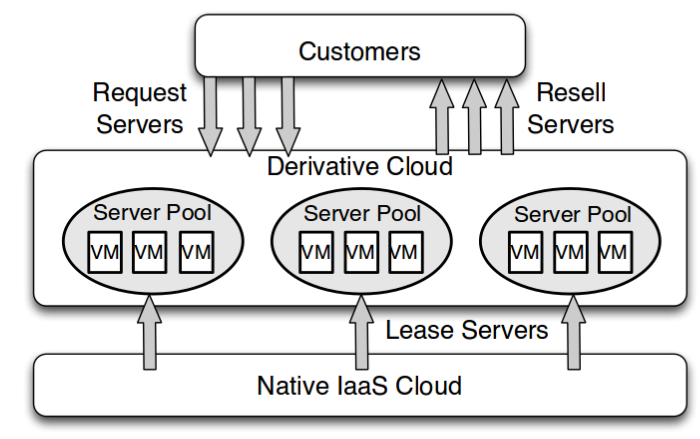
\includegraphics[width=0.7\textwidth]{images/derivative_cloud.png}
      \caption{Depiction of a derivative IaaS cloud platform, Source:\cite{sharma2015spotcheck}}
      \label{img_derivative_cloud}
    \end{figure}

    This idea of elastic provisioning can be expanded to a \textit{derivative cloud} environment as purposed by P.Sharma in his recent work 
\cite{sharma2015spotcheck} which repackages and resells resources purchased from native IaaS platforms. A derivative cloud can offer 
resources to customers with different pricing models and availability guarantees not provided by native platforms using a mix of resources  
purchased under different contract. Derivative cloud providers rent resources from native cloud providers to resell services to customers 
as shown in Fig:\ref{img_derivative_cloud}. Pi-Cloud\cite{picloud} and Heroku\cite{heroku} are examples derivative clouds that offer batch 
processing service and PaaS offerings respectively by repacking native Iaas services. 

    Although containers support has been provided in most major operating systems today, it is most popular and widely used in operating 
systems running on a Linux kernel. Our entire work would focus on elastic provisioning of containers in a native Linux environment and 
extend its implications to the derivative setup. However at this stage, we focus on elastic provisioning of memory as a resource. We aspire 
to look into other resources as a part of our future work.
   
    \subsection{Provisioning Memory as a Resource using Linux Containers}
  
      Memory as a resource has gained popularity recently with emergence of more memory intensive applications in various fields of 
computing like data analytics, caching that have a very strong correlation with application performance that is dependent on the memory 
available in the system. Most memory sensitive applications constantly use any unused memory available in the system to benefit them. A 
simple example is an Key-value used to cache frequent key's accessed by a web application. 

      Currently available provisioning knobs in the Linux container framework are quite effective while provisioning for applications when 
the host system isn't under any memory pressure and overcommitment (When resources promised on a system is more than resources available). 
However overcommitment is a fundamental requirement to provision cloud servers to maximize provider running costs as discussed earlier. In a 
native Linux system, memory pressure might be generated due to the following 

      \begin{enumerate}
	\item Additional memory required by processes of other containers
	\item More memory required by processes/services running on host Linux OS
	\item Memory pressure generated by kernel threads/processes
      \end{enumerate}
      
      Let's see how memory overcommitment and pressure can disrupt desired functionality of the existing container framework provided by 
Linux containers.
    
      \subsubsection{Illustrate existing problem}
	
	Consider two containers provisioned for running Mongo-DB containers from 2 different customers on a same host machines. Now that 
average memory used by the 2 containers are in the ratio of 1:2 and the customers for the 2 containers are also paying for their services in 
the same ratio. Let's call container with 1x workload usage as Mongo-Low and that of with 2x usage as Mongo-High. Now assume the customers 
have been provisioned using existing memory knobs with the same ratio as shown in Tab:\ref{table_initial}. For the sake of simplicity assume 
that all the containers over-provisioned for all other resources and aren't throttled by any other resource. Low and High can be thought of 
relative priorities of each of the containers.
	
	\vspace*{1em}	
	\begin{table}[!h]
	  \begin{center}
	    \begin{tabular}{ l | p{3cm} | p{2.2cm} | p{2.2cm} | p{2.2cm} }	      	    
		  & Average Memory Usage & Cost Paid for Service & Memory Provisioned & Desired Throughput \\ 
	      \hline
	      \hline
	      Mongo-Low  & 1x & 1x & 1x & 1x \\  
	      \hline
	      Mongo-High & 2x & 2x & 2x & 1x \\
		
	    \end{tabular}
	  \caption{Memory Provisioned for the Containers using existing memory provisioning knobs}
	  \label{table_initial}
	  \end{center}	  
	\end{table}
	\vspace*{1em}
	
	\pagebreak
	
	\begin{figure*}[t!]
	  \centering
	  \begin{subfigure}[t]{0.48\textwidth}
	    \centering
	    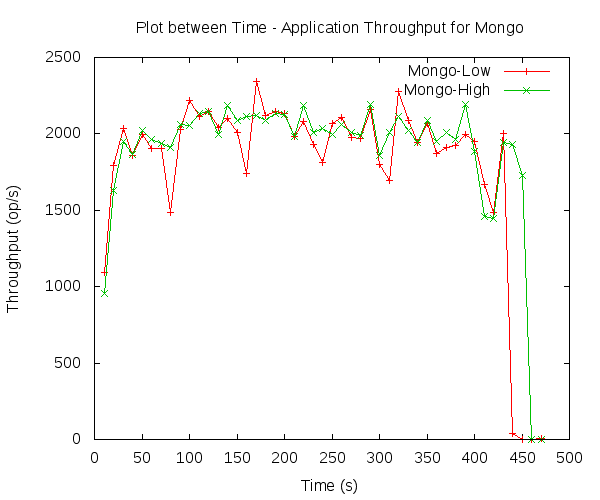
\includegraphics[width=1\textwidth]{images/intro/native.png}
	    \caption{App throughput when running applications natively}
	    \label{plot_intro_native}
	  \end{subfigure}
	  ~ 
	  \begin{subfigure}[t]{0.48\textwidth}
	    \centering
	    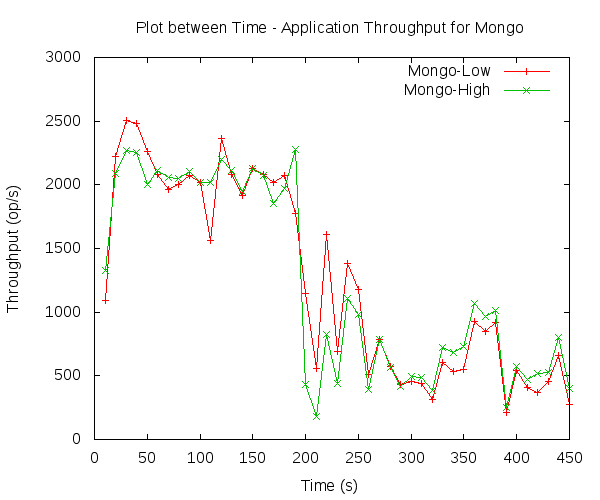
\includegraphics[width=1\textwidth]{images/intro/observed.png}
	    \caption{Observed throughputs after provisioning containers using existing knobs}
	    \label{plot_intro_observed}
	  \end{subfigure}
	  ~ 
	  \begin{subfigure}[t]{0.48\textwidth}
	    \centering
	    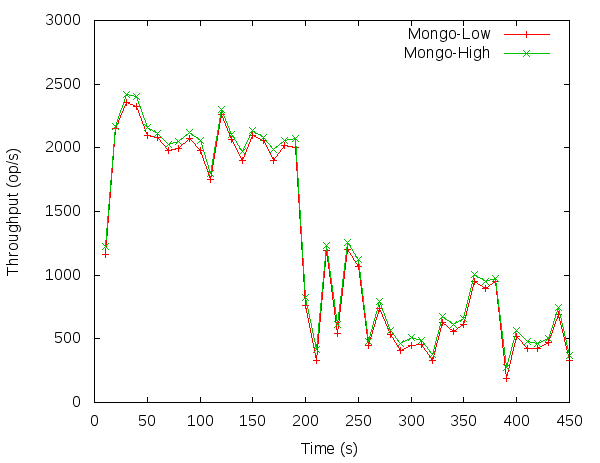
\includegraphics[width=1\textwidth]{images/intro/desired.png}
	    \caption{Desired throughputs after provisioning containers using existing knobs}
	    \label{plot_intro_desired}
	  \end{subfigure}
	  \caption{Plots for problem establishment}
	\end{figure*}
	
	Consider 3 cases as described below. In cases 2 and 3, containers are allowed to run normally for about 100s and there after 
which free memory in the system gradually reduces by generating of memory pressure by an external entity. 
	
	\begin{itemize}
	  \setlist{nosep,after=\vspace{\baselineskip}}
	  \item Case-1: Running applications natively in a system with 1:2 memory assignments and no pressure 
	  \item Case-2: Observed throughputs after provisioning with existing knobs under pressure
	  \item Case-3: Desired throughputs under pressure
	\end{itemize}
	
	Fig:\ref{plot_intro_native} shows the simple case where both the containers achieve desired throughputs when running on a system 
with no container specific provisioning. The containers start execution with no memory pressure and hence are able to each equal 
throughputs initially in all 3 cases. In observed throughputs under pressure Fig:\ref{plot_intro_observed}, we observe that throughputs of 
Mongo-High (Container with higher priority) is negatively affected at some point or the other, when in reality its throughput had to be 
better if not same as shown in Fig:\ref{plot_intro_desired} considering its higher resource allocations. 
	
	\pagebreak

	\begin{table}
	  \begin{center}
	    \begin{tabular}{ l | c | c | c }	      	    
		  & No Pressure & Observed & Desired \\ 
	      \hline
	      \hline
	      Mongo-Low  & 1825 & 1268 & 1255$-$ \\  
	      \hline
	      Mongo-High & 1972 & 1242 & 1255$+$ \\
		
	    \end{tabular}
	  \caption{Average throughput in each case (op/s)}
	  \label{table_intro_th}
	  \end{center}	  
	\end{table}
	
	Table:\ref{table_intro_th} shows how average throughputs vary in each case. It can be seen that the average throughput in case-2 
which is the provisioning of containers using existing knobs may negatively impact containers with higher allocations. By looking at the 
example here, we can conclude by saying that 
	
	\begin{enumerate}
	  \item Memory allocations work well with containers where there doesn't exist any memory overcommitment and pressure
	  \item However when the two occur, memory reclamation may adversely affects containers which are better provisioned (since they 
were promised higher QOS) than those which aren't.
	\end{enumerate}
    
    \subsection{Amplification of problem in derivative cloud environment}
    
      Considering the above described setup to derivative cloud where the native cloud provider is using VMs to provision customer demands. 
This VM acquired from the native cloud provider is again repacked and resold by the derivative cloud provider to specific customers. In 
this case, this situation further complicated due to two reasons,
      
       \begin{enumerate}
	  \item Memory overcommitment is not a required condition
	  \item Memory pressure maybe introduced by three factor described earlier or an external host system driver (eg: Balloon Driver)
       \end{enumerate}

      In the native case, memory overcommitment was a required condition for the previously described situation to arise. Consider the case 
where all containers were assigned memory considering the available system memory in such a way that there is no overcommitment, however 
now the native cloud provider (host system) could reduce the memory available to the system using different memory reclamation policies at 
the host. 

      The reclamation could be trigger by a host driver like the \textit{Balloon Driver} that is widely used by the \textit{Hypervisor} 
(Entity that manages VMs) by cloud providers. This leads to further discrepancies in the memory management at the container level. 
  
  \pagebreak
  
  \section{Problem Statement}
    
    This report presents the preliminary results of an empirical evaluation of memory management patterns in the native container 
environment and how this is affects real application in a derivative cloud environment. It tries to understand the following questions

    \begin{enumerate}
      \item How is memory management done for Linux containers ?
      \item What and when are the different types of memory management techniques invoked ?
      \item How do container memory configurations impact application performance ?
      \item What effect do the different container knobs have on the existing management policy ?
      \item Do existing knobs work as desired ?
    \end{enumerate}
    
    An comprehensive empirical evaluation which involves the above scenarios, and uses a set of workloads will help us understand the above 
questions. Once this has been established, we could move to purposing a solution to tackle the pitfalls of the existing approach.

  \section{Outline}
  
    This report is organized as follows, Chapter 2 provides the background required to read and understand the rest of the report, Chapter 
3 presents the design of the empirical evaluation, and Chapter 4 presents preliminary results.  Chapter 5 provides key insights to the 
desired system design. Chapter 6 concludes with the future work.

  